\documentclass[12pt]{article}

\usepackage{geometry}
\usepackage{amsmath,amsthm,amssymb}
\usepackage{graphicx}
\usepackage{multicol}
\usepackage{capt-of}

\newcommand{\lemma}{\noindent \textbf{Lemma: }}
\newcommand{\thm}{\noindent \textbf{Theorem: }}
\newcommand{\lskip}{\vspace{\baselineskip}}

\begin{document}

\title{Red-Black and 2-3-4 Trees}
\author{}
\maketitle

\section*{Description}
Red-black trees are loosely self-balanced BSTs. They have a 1-to-1 correspondence to 2-3-4 trees, and are easier and more efficient to implement; however, the theory behind the rebalancing is clearer to illustrate with 2-3-4 trees.

Compared to AVL trees, lookup times in a red-black tree are generally slower because they are less strictly balanced. However, insertion and deletion are generally faster because they require fewer rotations to rebalance the tree. In general red-black trees are used for language libraries (e.g. C++'s set and map) and AVL trees are used in databases, where fast lookups are preferred.

\section*{Properties}
2-3-4 trees have the following properties:
\begin{enumerate}
  \item Each node has either 2, 3, or 4 children (and 1 fewer key). \item The depth of every leaf node is the same.
\end{enumerate}

\noindent Red-black trees have the following properties.
\begin{enumerate}
  \item Nodes are colored red or black.
  \item The root is always black.
  \item No red node has a red child.
  \item \label{rb_desc_prop} Every path from a given node to each of its descendant leaves has the same number of black nodes.
\end{enumerate}
Note that by Property \ref{rb_desc_prop}, every root-to-leaf path has the same number of black nodes. We refer to this value as the \emph{black height} of the tree. The black height of a red-black tree is equal to the height of its corresponding 2-3-4 tree.

\section*{Insertion}
To insert into a red-black tree, we start with a normal BST insert and color the inserted node $N$ red. There are three cases for the position of $N$.
\begin{enumerate}
  \item $N$ is the root. In this case, we just color the insertednode the black and we have increase the black height of the tree by 1.
  \item $N$ has a black parent. In this case, the black height has not changed and no double red was created, so we are done.
  \begin{center}
    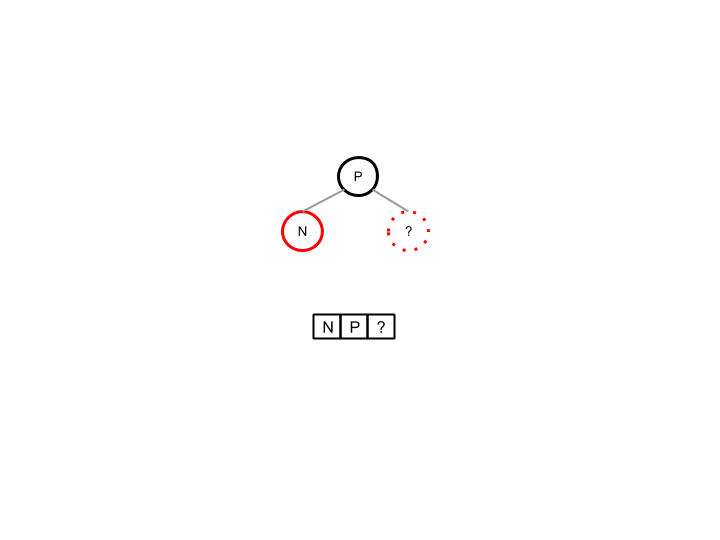
\includegraphics[scale=0.75]{pics/red_black_tree/ins_bpar}
    \captionof{figure}{Insertion where $N$ has a black parent}
  \end{center}
  \item $N$ has a red parent. Since the root is always black, we know a grandparent exists. This case is further divided into two cases:
  \begin{enumerate}
    \item $N$'s uncle is black or null. Note that $S$ must be a leaf, otherwise black height will not be constant. To rebalance, we simply perform an AVL rotation about the grandparent and recolor.
    \begin{center}
      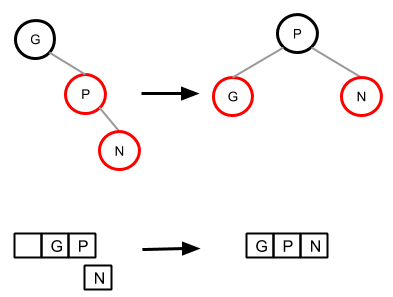
\includegraphics[scale=0.75]{pics/red_black_tree/ins_rpar_bunc_rr}
      \captionof{figure}{Insertion where $N$ has a red parent and black uncle: RR rotation}
    \end{center}
    \begin{center}
      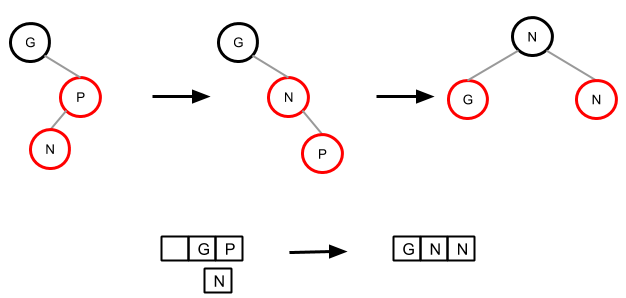
\includegraphics[scale=0.55]{pics/red_black_tree/ins_rpar_bunc_rl}
      \captionof{figure}{Insertion where $N$ has a red parent and black uncle: RL rotation}
    \end{center}
    \item $N$'s uncle is red. To rebalance, we color the parent and uncle black, color the grandparent red (if it is not the root), and then recurse on the grandparent if we created a double red. Note how this corresponds to ``pushing up'' a node in the 2-3-4 tree.
    \begin{center}
      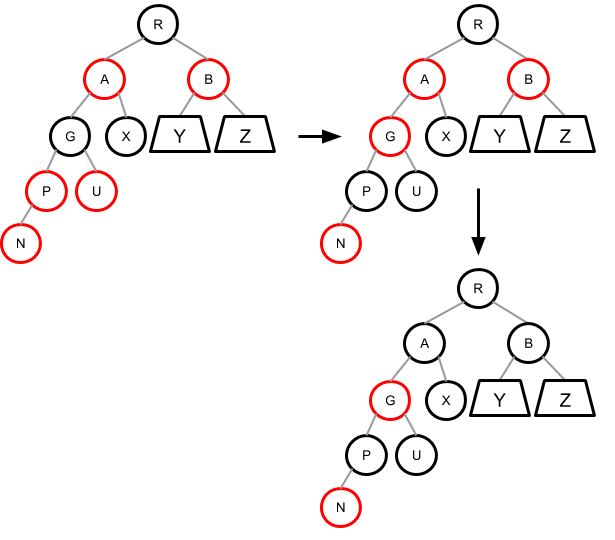
\includegraphics[scale=0.5]{pics/red_black_tree/ins_rpar_runc_rb}
      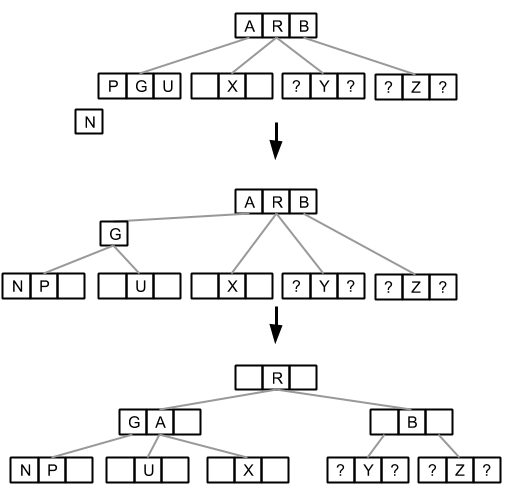
\includegraphics[scale=0.5]{pics/red_black_tree/ins_rpar_runc_234}
      \captionof{figure}{Insertion where $N$ has a red parent and red uncle}
      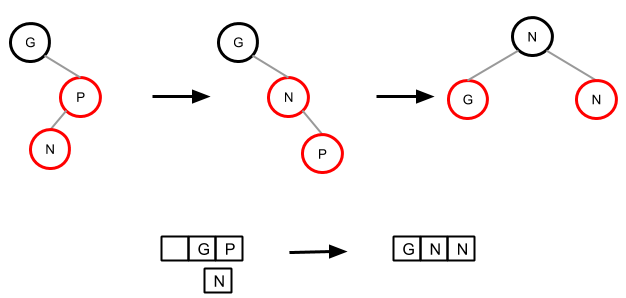
\includegraphics[scale=0.55]{pics/red_black_tree/ins_rpar_bunc_rl}
      \captionof{figure}{Insertion where $N$ has a red parent and black uncle: RL rotation}
    \end{center}
  \end{enumerate}
\end{enumerate}


\section*{Deletion}
For deletion, we once again start with a normal BST delete. Recall that in a BST deletion, the node we ultimately remove from the tree will either be a leaf or have only one child. However, if we are deleting a red node, it cannot have a single black child because the black height would be different between the left and right subtrees, and by rule, it cannot have a red child. That leaves us with three cases:

\begin{enumerate}
  \item Red leaf. The node can simply be removed without changing the black height.
  \begin{center}
    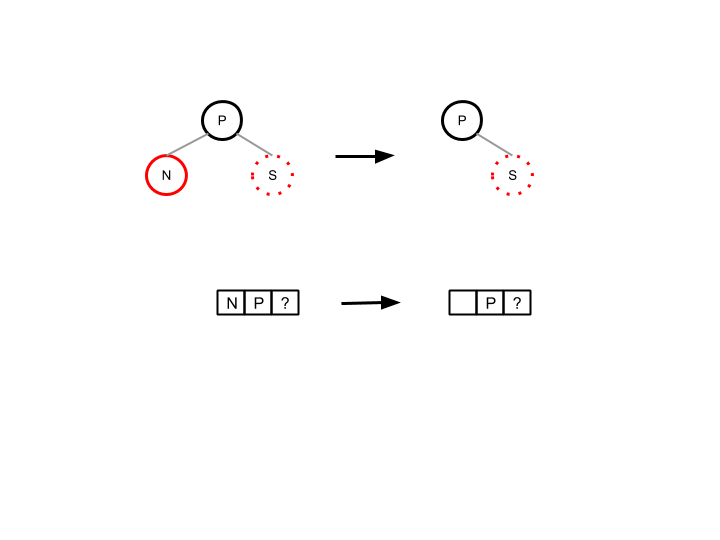
\includegraphics[scale=0.75]{pics/red_black_tree/del_red_leaf}
    \captionof{figure}{Deletion where $N$ is a red leaf}
  \end{center}

  \item Black node with a single child. Note that its child must be red to maintain a constant black height. We replace $N$ with the child and color the child black. The black height of the tree does not change.
  \begin{center}
    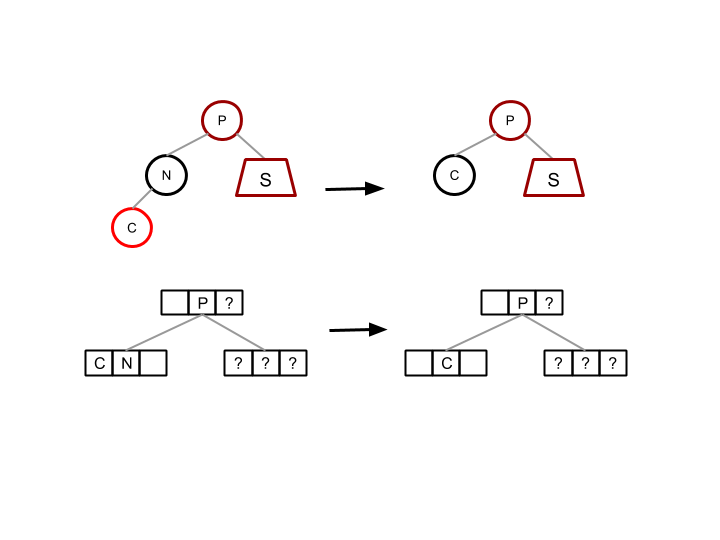
\includegraphics[scale=0.7]{pics/red_black_tree/del_black_red_child}
    \captionof{figure}{Deletion where $N$ is a black node with a single child}
  \end{center}

  \item Black leaf. This case is further divided into three cases.
  \begin{enumerate}
    \item \label{bleaf_bsib1} $N$ has a black sibling and a red nephew. $N$ is a leaf, so ? must be red or null to maintain constant black height. To rebalance, we perform an AVL rotation about the parent and recolor.
    \begin{center}
      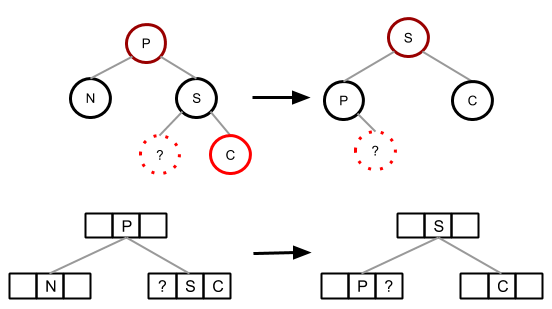
\includegraphics[scale=0.65]{pics/red_black_tree/del_bleaf_bsib_rneph_rr}
      \captionof{figure}{Deletion where $N$ is a black leaf and has a black sibling and a red nephew: RR rotation}
    \end{center}
    \begin{center}
      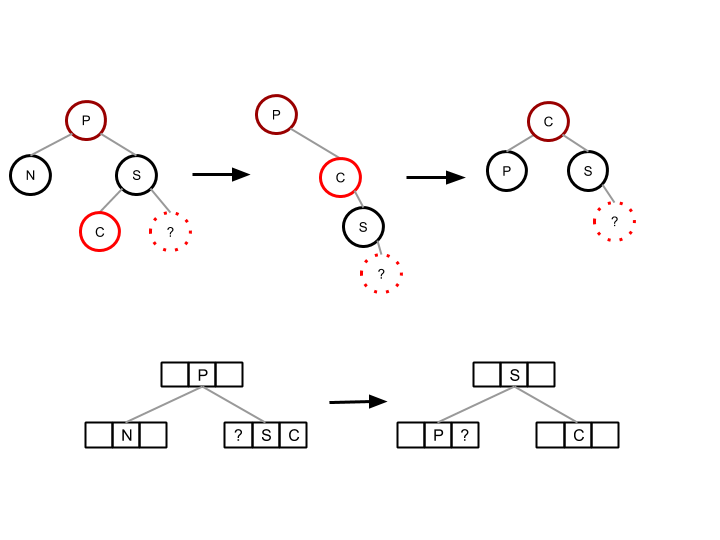
\includegraphics[scale=0.55]{pics/red_black_tree/del_bleaf_bsib_rneph_rl}
      \captionof{figure}{Deletion where $N$ is a black leaf and has a black sibling and a red nephew: RL rotation}
    \end{center}

    \item \label{bleaf_bsib2} $N$ has a black sibling and no red nephews. Here, we color the sibling red and the parent black. Then, we recurse parent on if it was already black and is not the root. Note that there is no risk of double red because both children are black or null.
    \begin{center}
      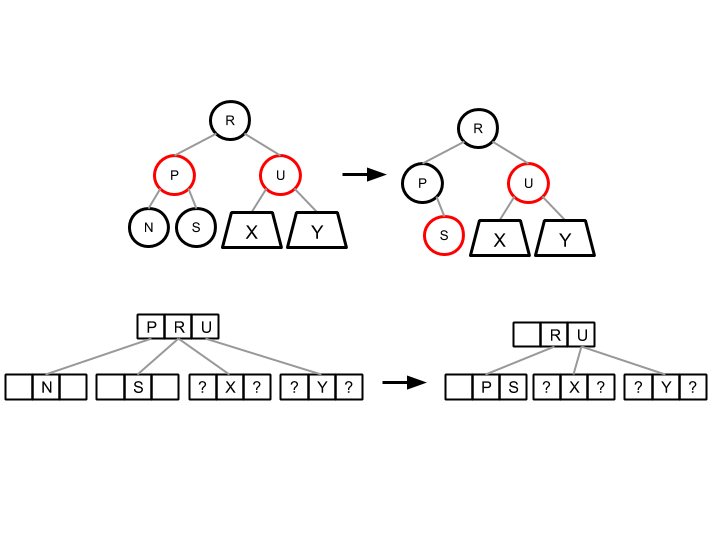
\includegraphics[scale=0.5]{pics/red_black_tree/del_bleaf_bsib_bnephs_rpar}
      \captionof{figure}{Deletion where $N$ has a black sibling, no red nephews, and a red parent}
    \end{center}
    \begin{center}
      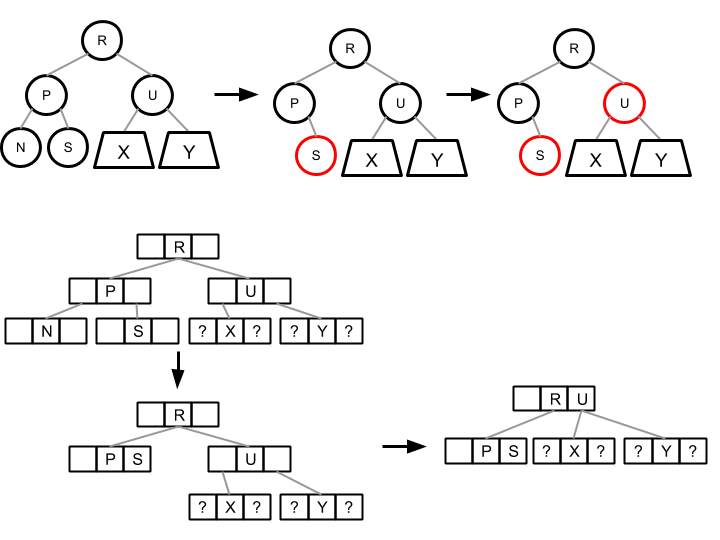
\includegraphics[scale=0.5]{pics/red_black_tree/del_bleaf_bsib_bnephs_bpar}
      \captionof{figure}{Deletion where $N$ is a black leaf and has a black sibling, no red nephews, and a black parent}
    \end{center}

    \item $N$ has a red sibling. Note that $P$ has to be black to prevent a double red. Also, $X$ and $Y$ must be non-null, black and have no black children because the black height is 2. To rebalance, we perform a normal rotation about $P$, color $P$ red, and color $S$ black. Now we have a valid tree and we are deleting a black leaf with a black sibling, so we can proceed to case \ref{bleaf_bsib1} or \ref{bleaf_bsib2}.
    \begin{center}
      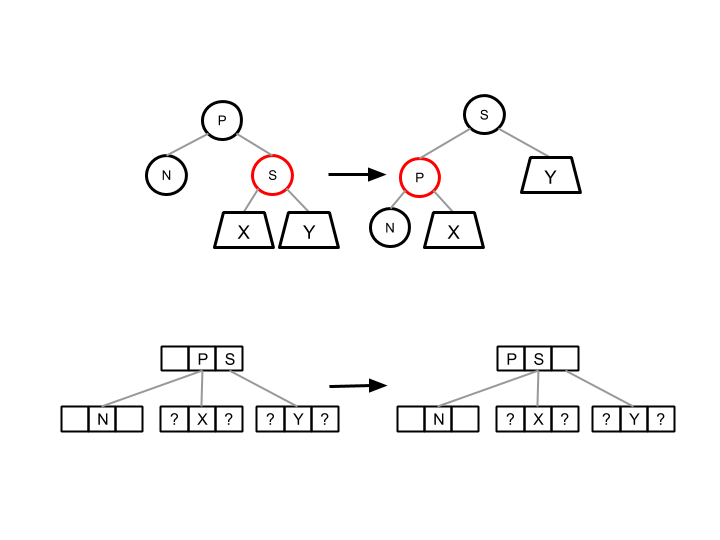
\includegraphics[scale=0.55]{pics/red_black_tree/del_bleaf_rsib}
      \captionof{figure}{Deletion where $N$ is a black leaf and has a red sibling}
    \end{center}

\end{enumerate}
\end{enumerate}

\section*{Time Complexity}

\end{document}
